\section{Konsole}
\label{sec:DesignKonsole}
Das Projekt CKi ist in seinem Grundaufbau für die Konsole konzipiert. Der grundlegende Befehl soll wie folgt aussehen: 
\begin{lstlisting}[language=bash]
	$ ki [options] [file]
\end{lstlisting}
Dabei gibt es drei Ausführungen von diesem Befehl.

\subsection{Training}
\label{sec:DesignTraining}
\subsubsection{Input}
\label{sec:DesignTraiInput}
\begin{lstlisting}[language=bash]
	$ ki --training [file]
	$ #Dieser Befehl nimmt ubyte-Dateien.
\end{lstlisting}

\subsubsection{Output}
\label{sec:TraiOutput}
Nach jedem Datensatz wird angezeigt, wie viele der zum Training gegebenen Daten bereits abgearbeitet wurden. 

\subsection{Verify}
\label{sec:DesignTest}
\subsubsection{Input}
\label{sec:DesignTestInput}
\begin{lstlisting}[language=bash]
	$ ki --verify [file]
	$ #Dieser Befehl nimmt ubyte-Dateien.
\end{lstlisting}

\subsubsection{Output}
\label{sec:TestOutput}
Nach jedem Datensatz wird angezeigt, wie viele der zum Testen gegebenen Daten bereits abgearbeitet wurden. Zudem wird angezeigt, wie viele der Datensatz richtig, genauer gesagt falsch erkannt wurden. 
\\
Eine interessante Erweiterung wäre es, bei diesem Befehl (oder in einer leicht abgewandelten Form) ein kleines Fenster zu öffnen, um dort direkt die Zahl zu zeichnen. Dies hätte den Vorteil, dass Parameter wie Grösse direkt bekannt und kontrolliert werden können.

\subsection{Prediction}
\label{sec:DesignAnwendung}
\subsubsection{Input}
\label{sec:DesignUseInput}
\begin{lstlisting}[language=bash]
	$ ki [file]
	$ #Dieser Befehl nimmt jpg-Dateien.
\end{lstlisting}

\subsubsection{Output}
\label{sec:DesignUseOutput}
Als Output werden alle Ziffern von 0 bis 9 mit den entsprechenden Prozentwerten zurückgegeben (Dies kommt daher, dass die KI die Wahrscheinlichkeit der Übereinstimmung für jede Ziffer berechnet.). Zudem wird auch angezeigt, welche Ziffer die höchste Übereinstimmung hat. Da diese die erkannte Ziffer darstellt.

\section{Datenbank}
\label{sec:DesignDatenbank}
Die Applikation benötigt keine Datenbank. Zur Speicherung der Test- und Trainings-Datensätze werden sogenannte ubyte-Dateien eingesetzt. Diese enden auf der Dateierweiterung „.ubyte“.

\subsection{UByte}
\label{sec:UByte}
Die Bilddateien im MNIST-Datensatz werden im sogenannten „ubyte“ (unsigned byte) Format gespeichert. Dies bedeutet, dass die Pixelwerte der Bilder als Bytes gespeichert werden. Jedes Bild im Datensatz wird als Reihe von Bytes dargestellt, wobei jedes Byte den Graustufenwert eines Pixels repräsentiert. Hinzu kommt, dass auch die dazugehörigen Labels in einer „ubyte“-Datei gespeichert werden.
\\
Aufgrund dieser Speicherung müssen die Datensets vor deren Verwendung eingelesen und interpretiert werden. 
\\
Für diese Interpretation muss die standardisierte Höhe und Weite für jedes auszulesende Bild multipliziert werden. Danach müssen so viele Bytes aus der entsprechenden „ubyte“-Datei ausgelesen werden und als vorzeichenlose ganze Zahlen gespeichert. Denn jede dieser Zahlen stellt einen Pixel dar.

Für eine genaue Anleitung für das Einlesen und Interpretieren in Python ist die Webseite \href{https://androidkt.com/extract-images-from-mnist-idx3-ubyte-file-format-in-python/}{AndroidKT} zu kontaktieren.

\begin{figure}[H]
	\centering
	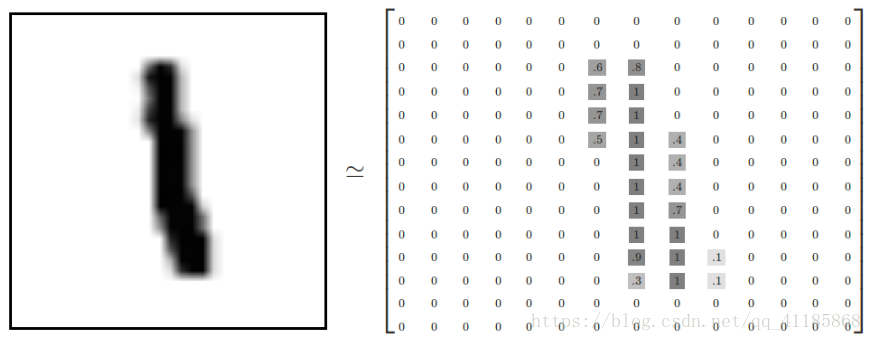
\includegraphics[width=\linewidth]{20180624202122600.png}
	\caption{Darstellung einer Ziffer und deren Code von \href{https://blog.csdn.net/qq_41185868/article/details/79094752}{blog.csdn.net}}
	\label{fig:designubytecomp}
\end{figure}



\section{Code}
\label{sec:DesignCode}
\subsection{Klassendiagramm}
\label{sec:DesignKlassendiagramm}
Es gibt vier Klassen im Projekt CKi. Dabei handelt es sich um auf sich selbst aufbauende Strukturen. Als Code-Einstieg fungiert die Main-Klasse, welche die Main-Funktion bereitstellt. In dieser wird die Klasse „Network“ aufgesetzt. Es werden mehrere Hidden-Layer erstellt, die Datensätze der MNIST-Datenkollektion eingelesen und die Funktionen „Train“ und „Predict“ sowie „Save Weights“ ausgeführt. 
\\
In der Network-Klasse werden mehrere Layer initialisiert und verwendet. Diese Layer sind in der Layer-Klasse definiert und besitzen wiederum multiple Neuronen.
\\
Die Neuronen sind die Knotenpunkte, welche mit der mathematischen Sigmoid-Funktion einen Output-Wert berechnen. Zusätzlich ermitteln diese auch die Fehler-Abweichung bei der Backpropagation, um die einzelnen Werte anzupassen.
\\
Um Sigmoid und die Ableitung von Sigmoid zu berechnen, gibt es noch eine Utility-Klasse „Util“. Diese besteht nur aus statischen Funktionen, welche an anderen Orten benötigt werden.


\begin{figure}[H]
	\centering
	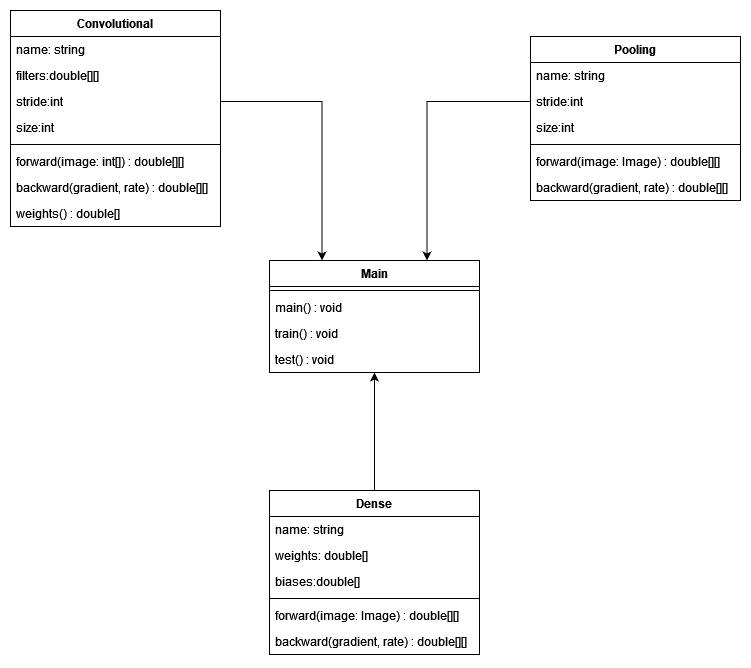
\includegraphics[height=0.5\paperheight]{Klassendiagramm.png}
	\caption{Das Klassendiagramm, Grundaufbau der Applikation}
	\label{fig:designklassendiagramm}
\end{figure}

\subsection{Trainingsdaten}
\label{sec:DesignTrainingsdaten}
Die Trainingsdaten sind das MNIST-Datenset mit den handschriftlichen Zahlen. (\url{http://yann.lecun.com/exdb/mnist/})

\subsection{Tests}
\label{sec:DesignTests}
Im Projekt CKI gibt es drei Arten von Tests. Es gibt das simple Ausprobieren. Da es nicht allzu viele Nutzerschnittstellen gibt, kann man diese ausführen und begutachten, ob diese mit der Beschreibung übereinstimmen.
Bei einer dieser Schnittstellen wird die KI getestet. Dies geschieht, indem die KI ihre unbekannten Datensätze zu sehen bekommt und das Endergebnis mit einem vordefinierten Ergebnis abgeglichen wird.
Egal, ob das Ergebnis korrekt oder inkorrekt erkannt worden ist, wird es statistisch aufgenommen. Am Ende wird dem Nutzer eine Prozentzahl der korrekten Erkenntnisse präsentiert. Diesbezüglich ist dies kein Test, in dem die Applikation versagen könnte, es ist eine reine Leistungsüberprüfung, ob mehr Training vonnöten ist.
Zusätzlich zu diesen zwei Testmöglichkeiten gibt es noch die Unit-Tests. Diese werden dazu genützt, um einzelne Funktionen und Klassen noch vor deren Verwendung zu überprüfen.
\\
Zusätzlich gegenüber diesen drei Tests wäre es überaus interessant zu begutachten und zu vergleichen, wie hoch die Leistungsunterschiede zwischen CKi und einem in Python mit TensorFlow gebauten Programm mit vergleichbarer Grundstruktur sind. Diesbezüglich wird neben CKi auch ein kleines vergleichbares Modell in Python realisiert, um diese Daten zu sammeln.



